\chapter{Q-iteration}\label{App:Q-iteration}


\section{Introduction}

This Appendix shows the results of the model-based approach to solve a \ac{RL} problem using \ac{LLR} as a model. This approach was tried for two reasons. First, we wanted to use the model-based policies as a benchmark result to which the model-free and model-learning methods could be compared. Furthermore, we searched for a way to compare \ac{LLR} to the true system. Since iterative methods do not use exploration, the results are always the same and therefore easy to compare. In this way it would be easy to compare for instance the number of memory samples on the quality of the model and the resulting policy.

\section{Experimental setup}
The results are obtained using Q-iteration in a learning problem using the two-link manipulator (Section \ref{sec:LLR-two link manipulator}). Q-iteration (Section \ref{sec:RL-Q_iteration}) is a model-based solution method that iterates over all states and actions to find a policy for the entire state-action space. The learning goal was to move the manipulator to 0. The reward was +10 for goal states and -1 elsewhere. We compared the results from the nonlinear model to the \ac{LLR} model of the system. The results were obtained using Q-iteration and Fuzzy approximation of the value function \cite{Busoniu:10}. The \ac{LLR} model was obtained by using a memory consisting of $7.5\cdot10^4$ samples, using $K=5$ nearest neighbors. These samples were distributed evenly over the state-space and were generated using the nonlinear model.


\paragraph{Performance measure}
Quality of an obtained policy and thus the performance of the model was assessed in two ways:
\begin{enumerate}
	\item \textbf{Visual inspection of the policy:} The policy obtained for the noiseless case (Figure \ref{fig:Q-iteration-subfig1a}) is taken as the 'true' policy. The noisy and \ac{LLR} policies should look similar to the true policy.
	\item \textbf{Discounted reward $J$:} A set of 100 initial states is generated evenly over the state-space and the obtained policy is used to simulate trajectories starting from these initial states. The mean of the discounted rewards obtained in these trajectories is a measure for how good the obtained policy is (higher reward equals better policy).
	$$
		J = \frac{1}{100}\sum_{i=1}^{100}{J_i}
	$$
\end{enumerate}


\section{Results}
\figref{fig:Q-iteration-results} shows the results obtained for Q-iteration applied on the two-link manipulator setup. The figures show the policy for the torques $\tau_1$ and $\tau_2$ in the two joints for $\omega_1=0$ and $\omega_2=0$.

The optimal result is the nonlinear model without noise. This result is shown in \figref{fig:Q-iteration-subfig1a}. The policy shows no artifacts and the performance of this policy is $J = -85.5$. The policy of the \ac{LLR} model for the noise-free case is shown in \figref{fig:Q-iteration-subfig1b}. The policy still looks reasonably good, but the performance $J=-104.8$ is much worse than for the nonlinear model.

For both cases the policy becomes worse when a white noise signal is added to the output of the model. The nonlinear model still performs reasonably well for a noise signal with $\sigma^2 = 0.01$, but deteriorates for increasing noise. The \ac{LLR} model also decreases in performance for increasing noise. In theory, the \ac{LLR} model could decrease the effect of noise. However, this is not supported by these results as the \ac{LLR} model always performs worse than the nonlinear model.

Several more experiments were carried out (not shown here) with various settings. The overall conclusions are the same for all cases: Adding noise quickly deteriorates the quality of the resulting policy and \ac{LLR} never leads to better results than the nonlinear model. Even a very large memory consisting of $3\cdot10^5$ samples, did not lead to good results. This surprising as the earlier modeling experiments \ref{sec:LLR-two link manipulator} showed very good modeling accuracy for only a few thousand samples.
\begin{figure}[ht]
	\centering
	\subfigure[nonlinear model, no noise, $J=-85.5$ ]{
	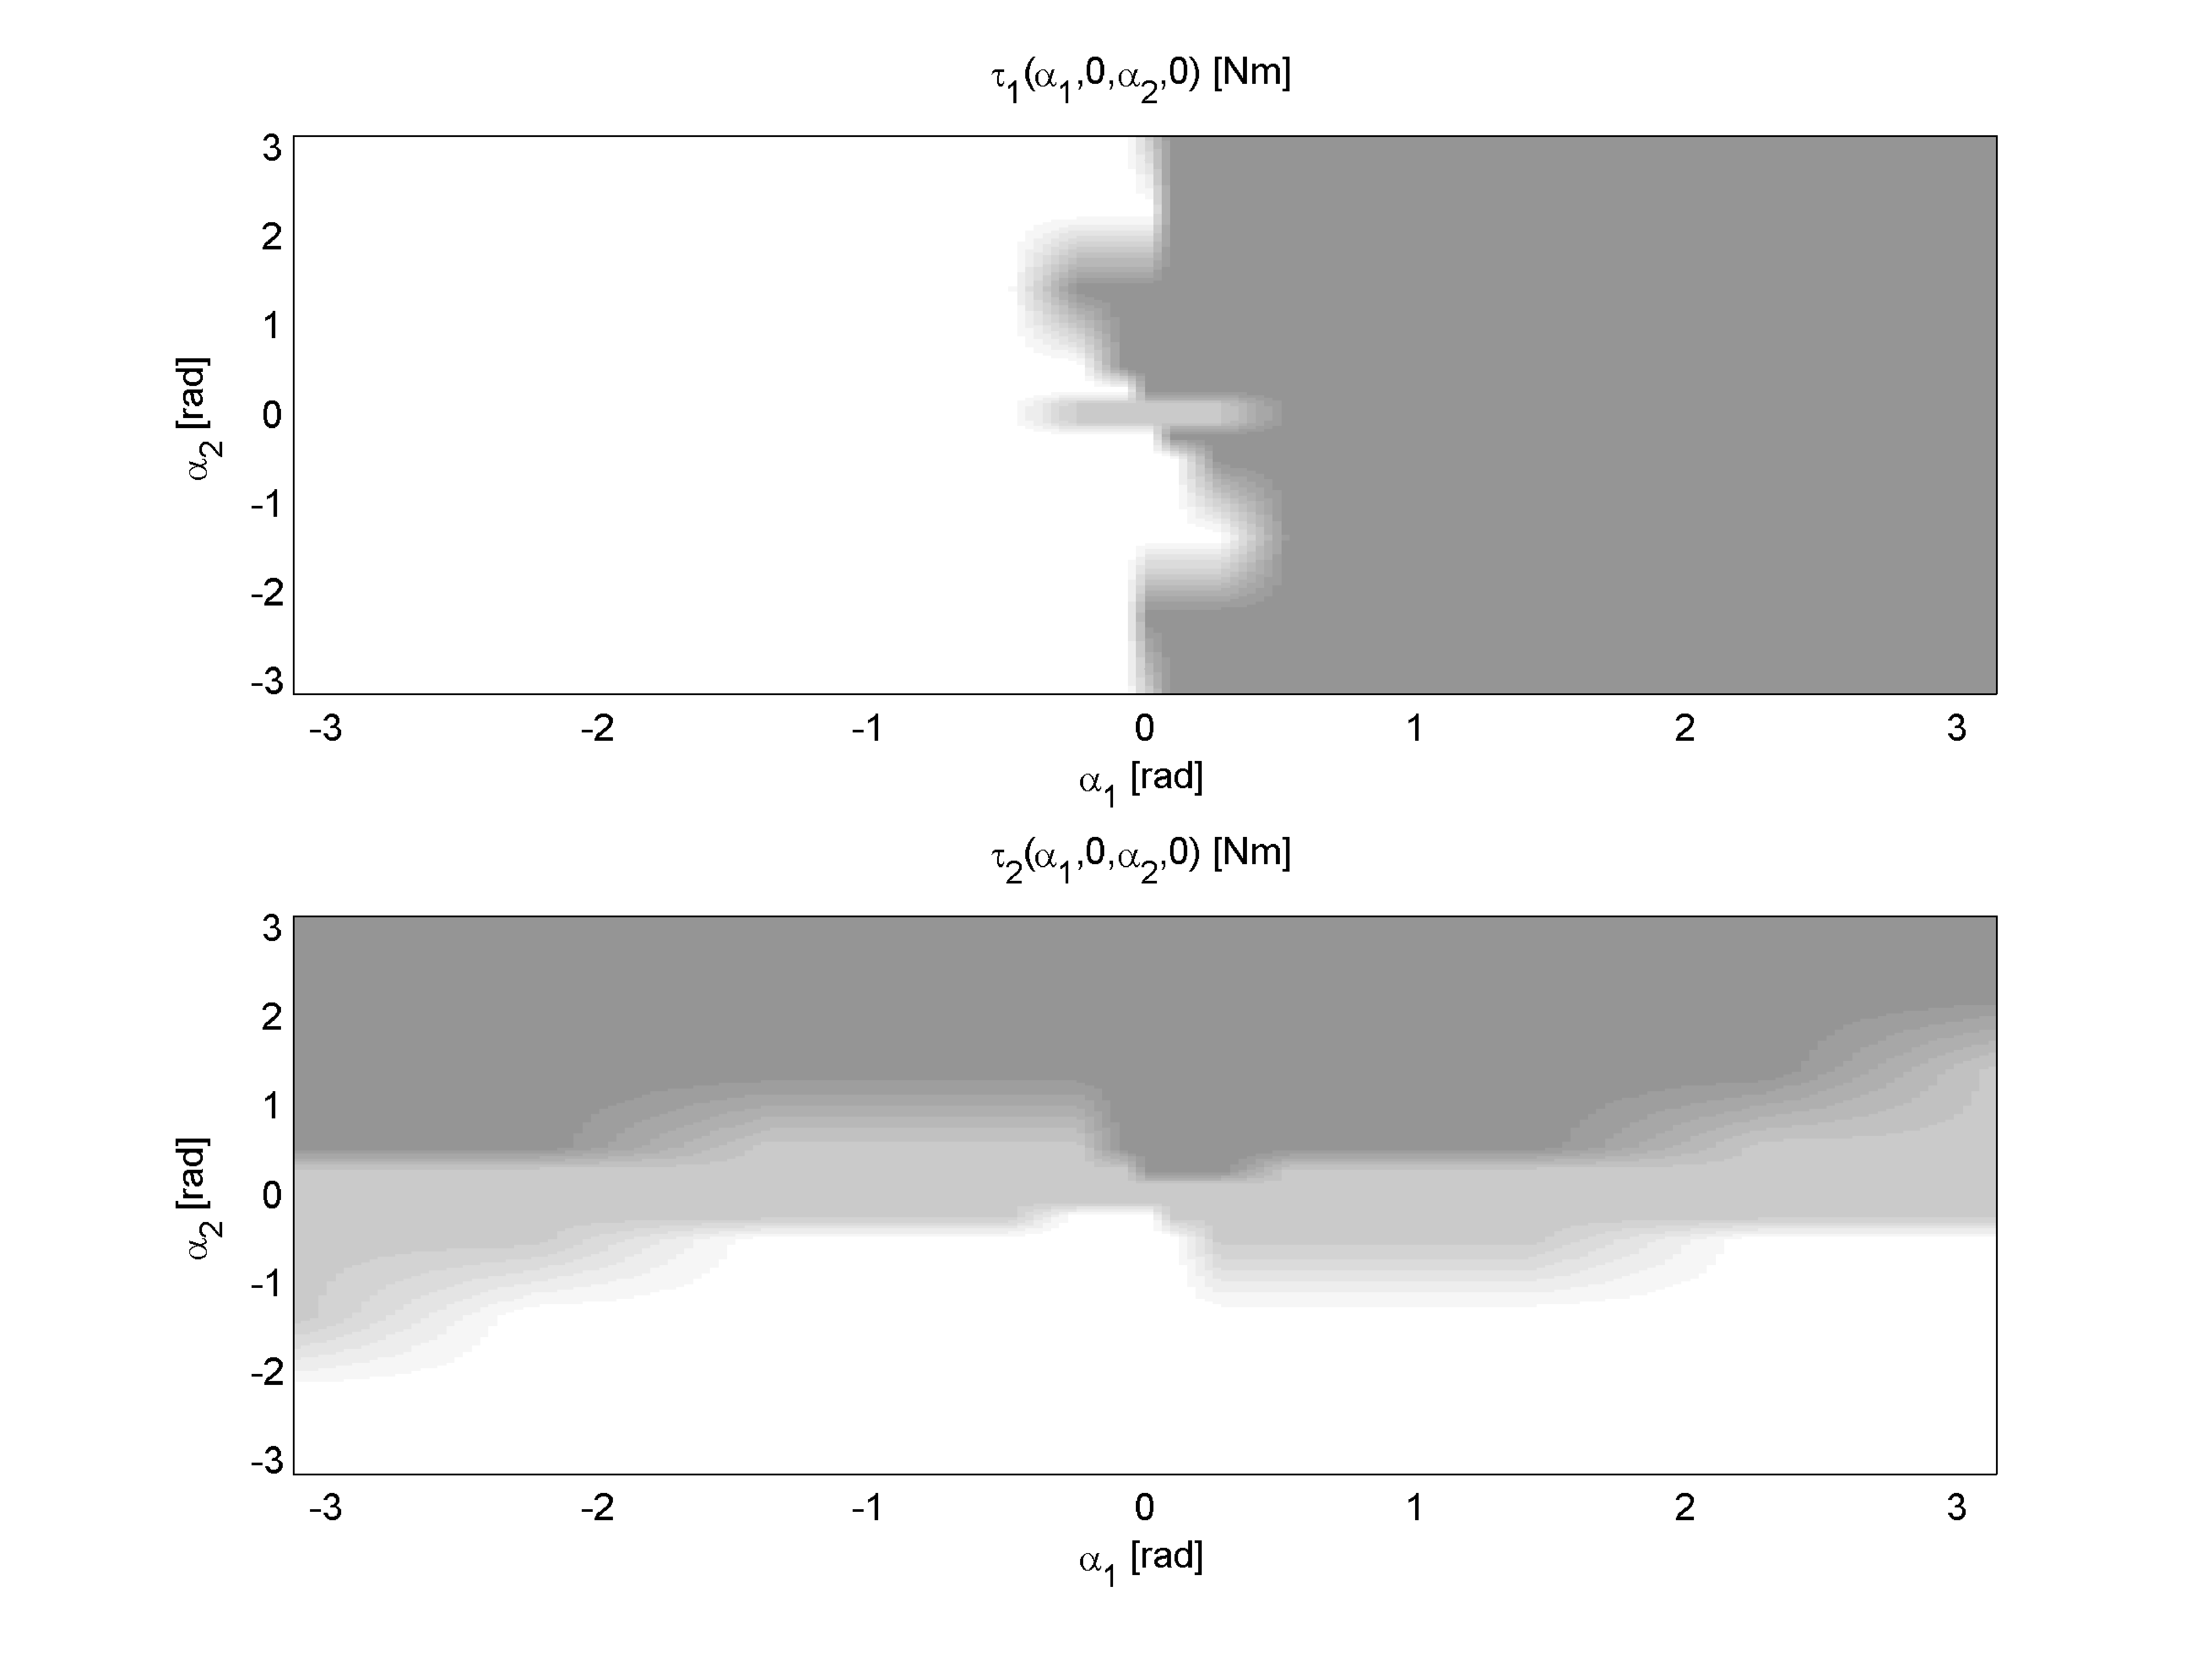
\includegraphics[width=.4\textwidth]{Figures/rarm_fzqi_test_1_fuzzyh.eps}
	\label{fig:Q-iteration-subfig1a}
	}
	\subfigure[LLR model, no noise, $J=-104.8$ ]{
	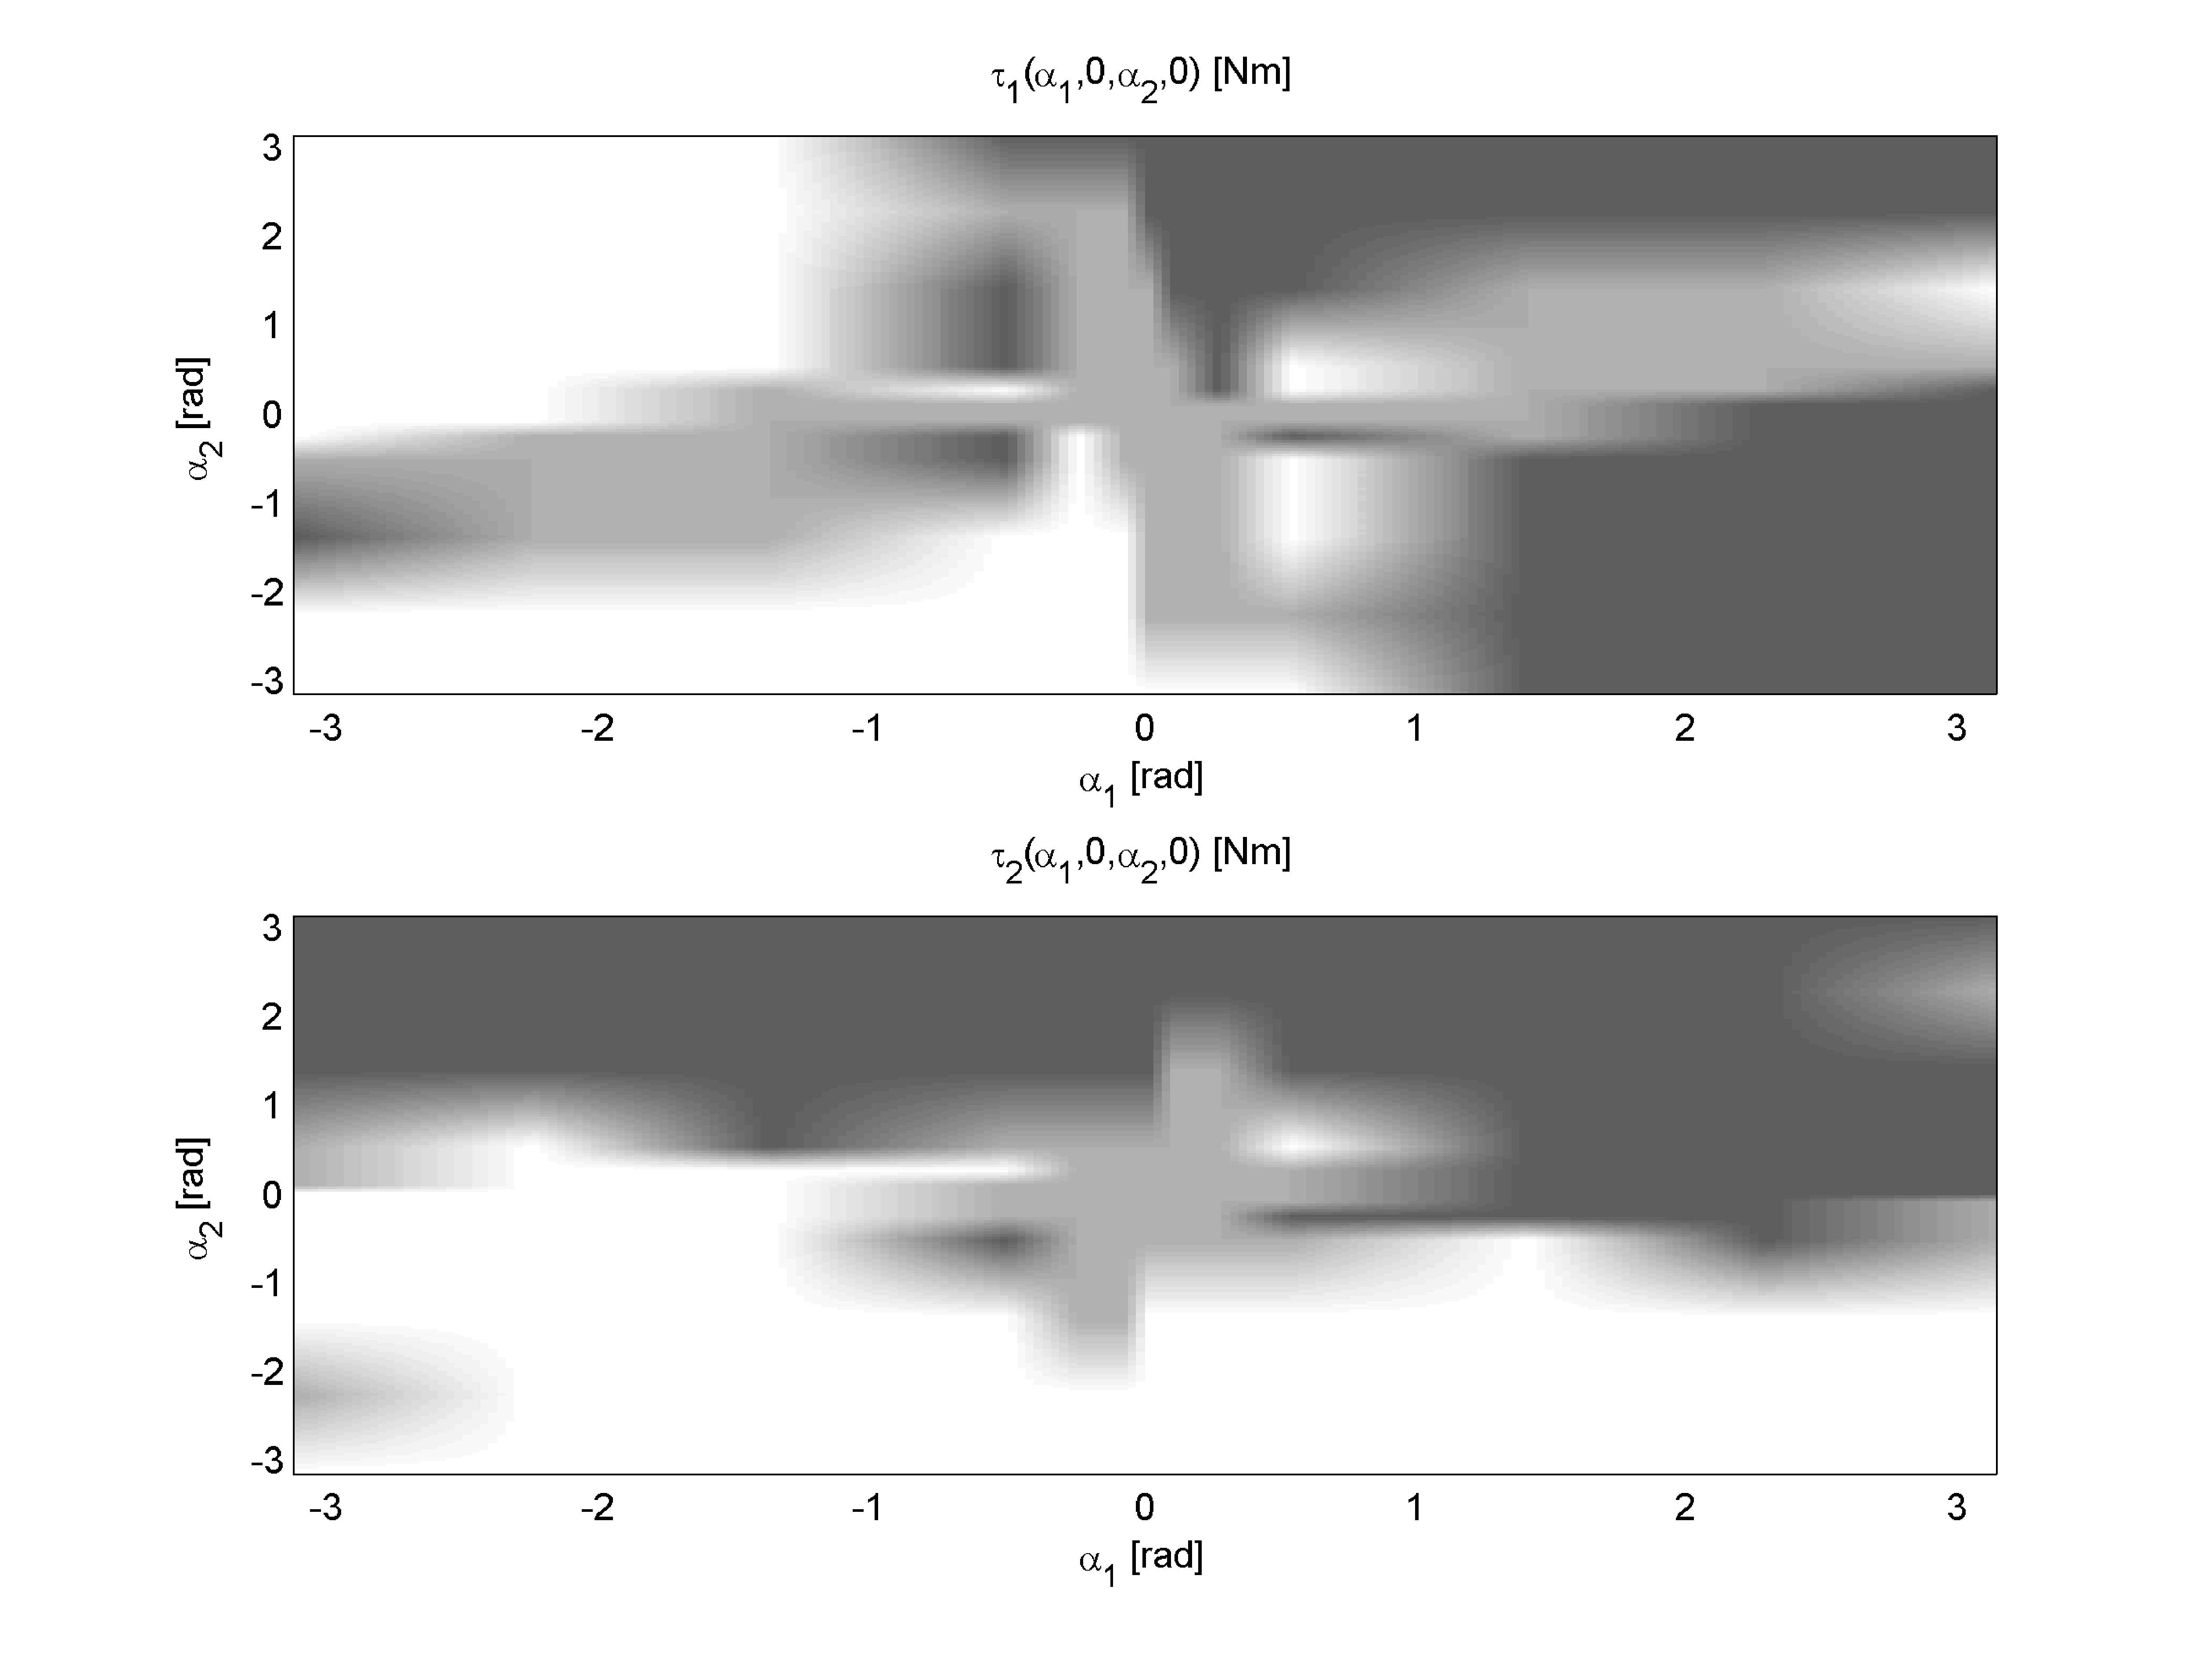
\includegraphics[width=.4\textwidth]{Figures/rarm_fzqi_LLR_test_1_fuzzyh.eps}
	\label{fig:Q-iteration-subfig1b}
	}
	\\
	\subfigure[nonlinear model, noise ($\sigma^2=0.01$), $J=-96.4$]{
	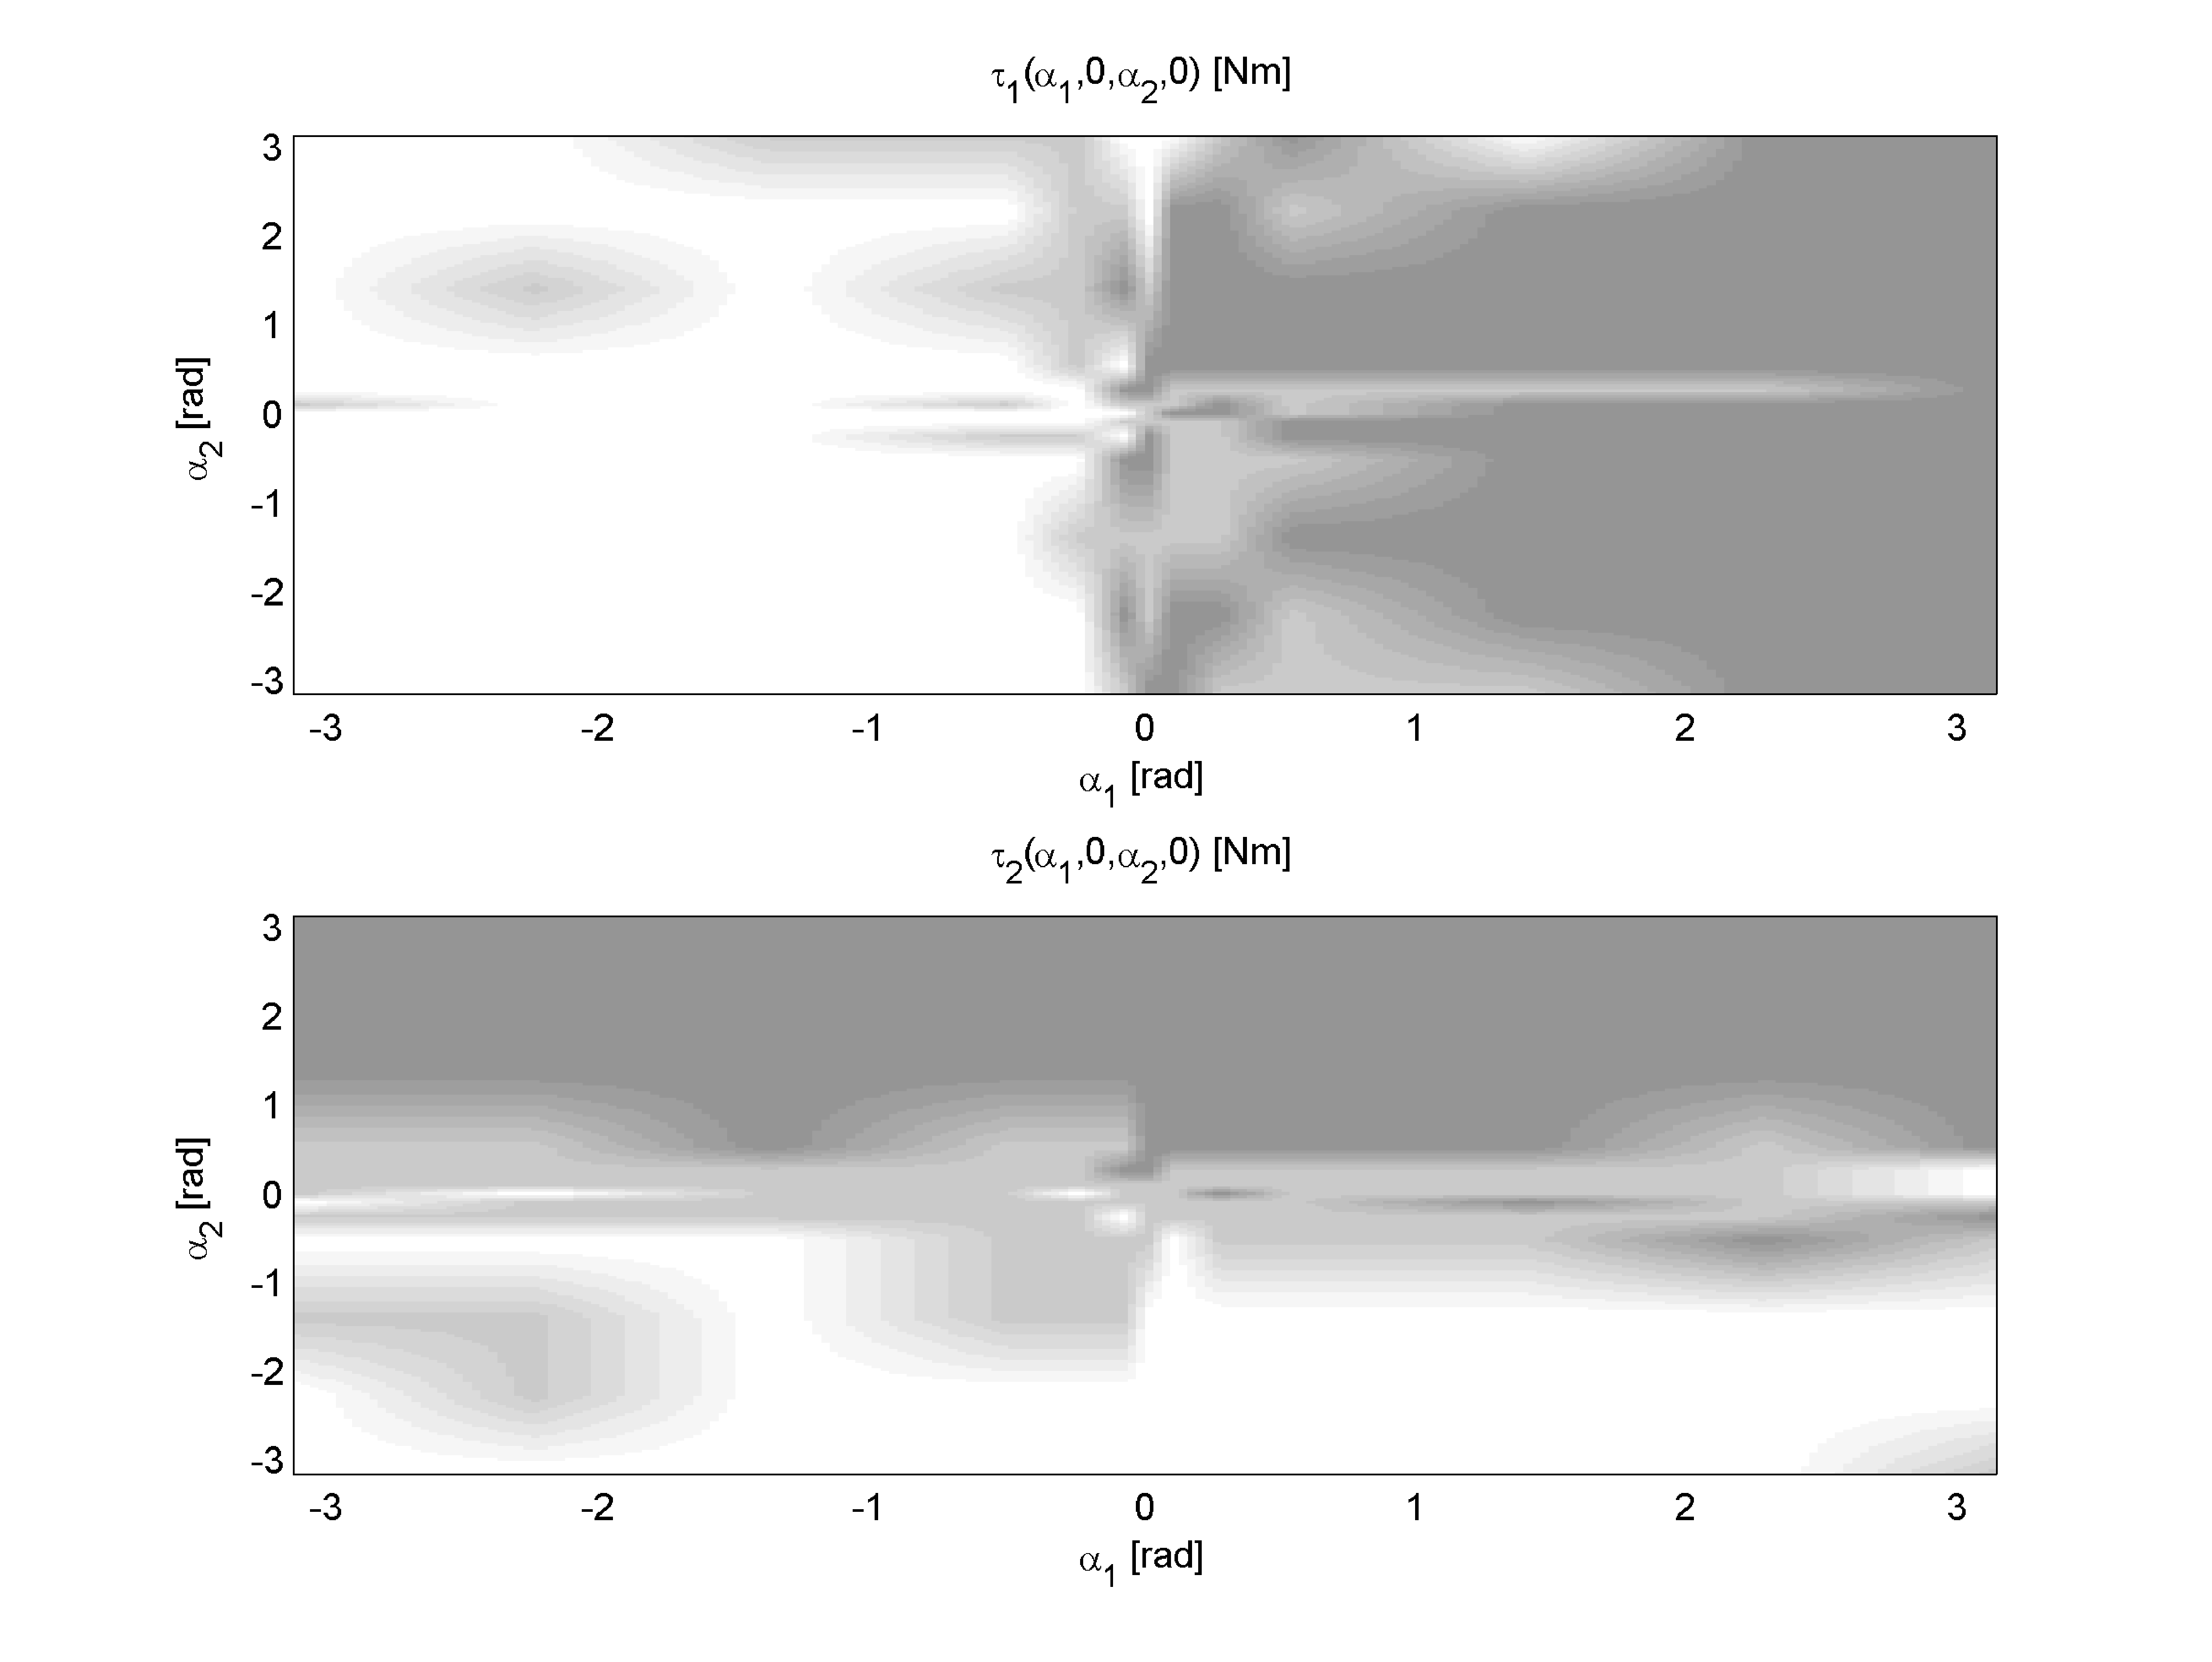
\includegraphics[width=.4\textwidth]{Figures/rarm_fzqi_test_1_noise_001_fuzzyh.eps}
	\label{fig:Q-iteration-subfig2a}
	}
	\subfigure[LLR model, noise ($\sigma^2=0.01$), $J=-133.5$]{
	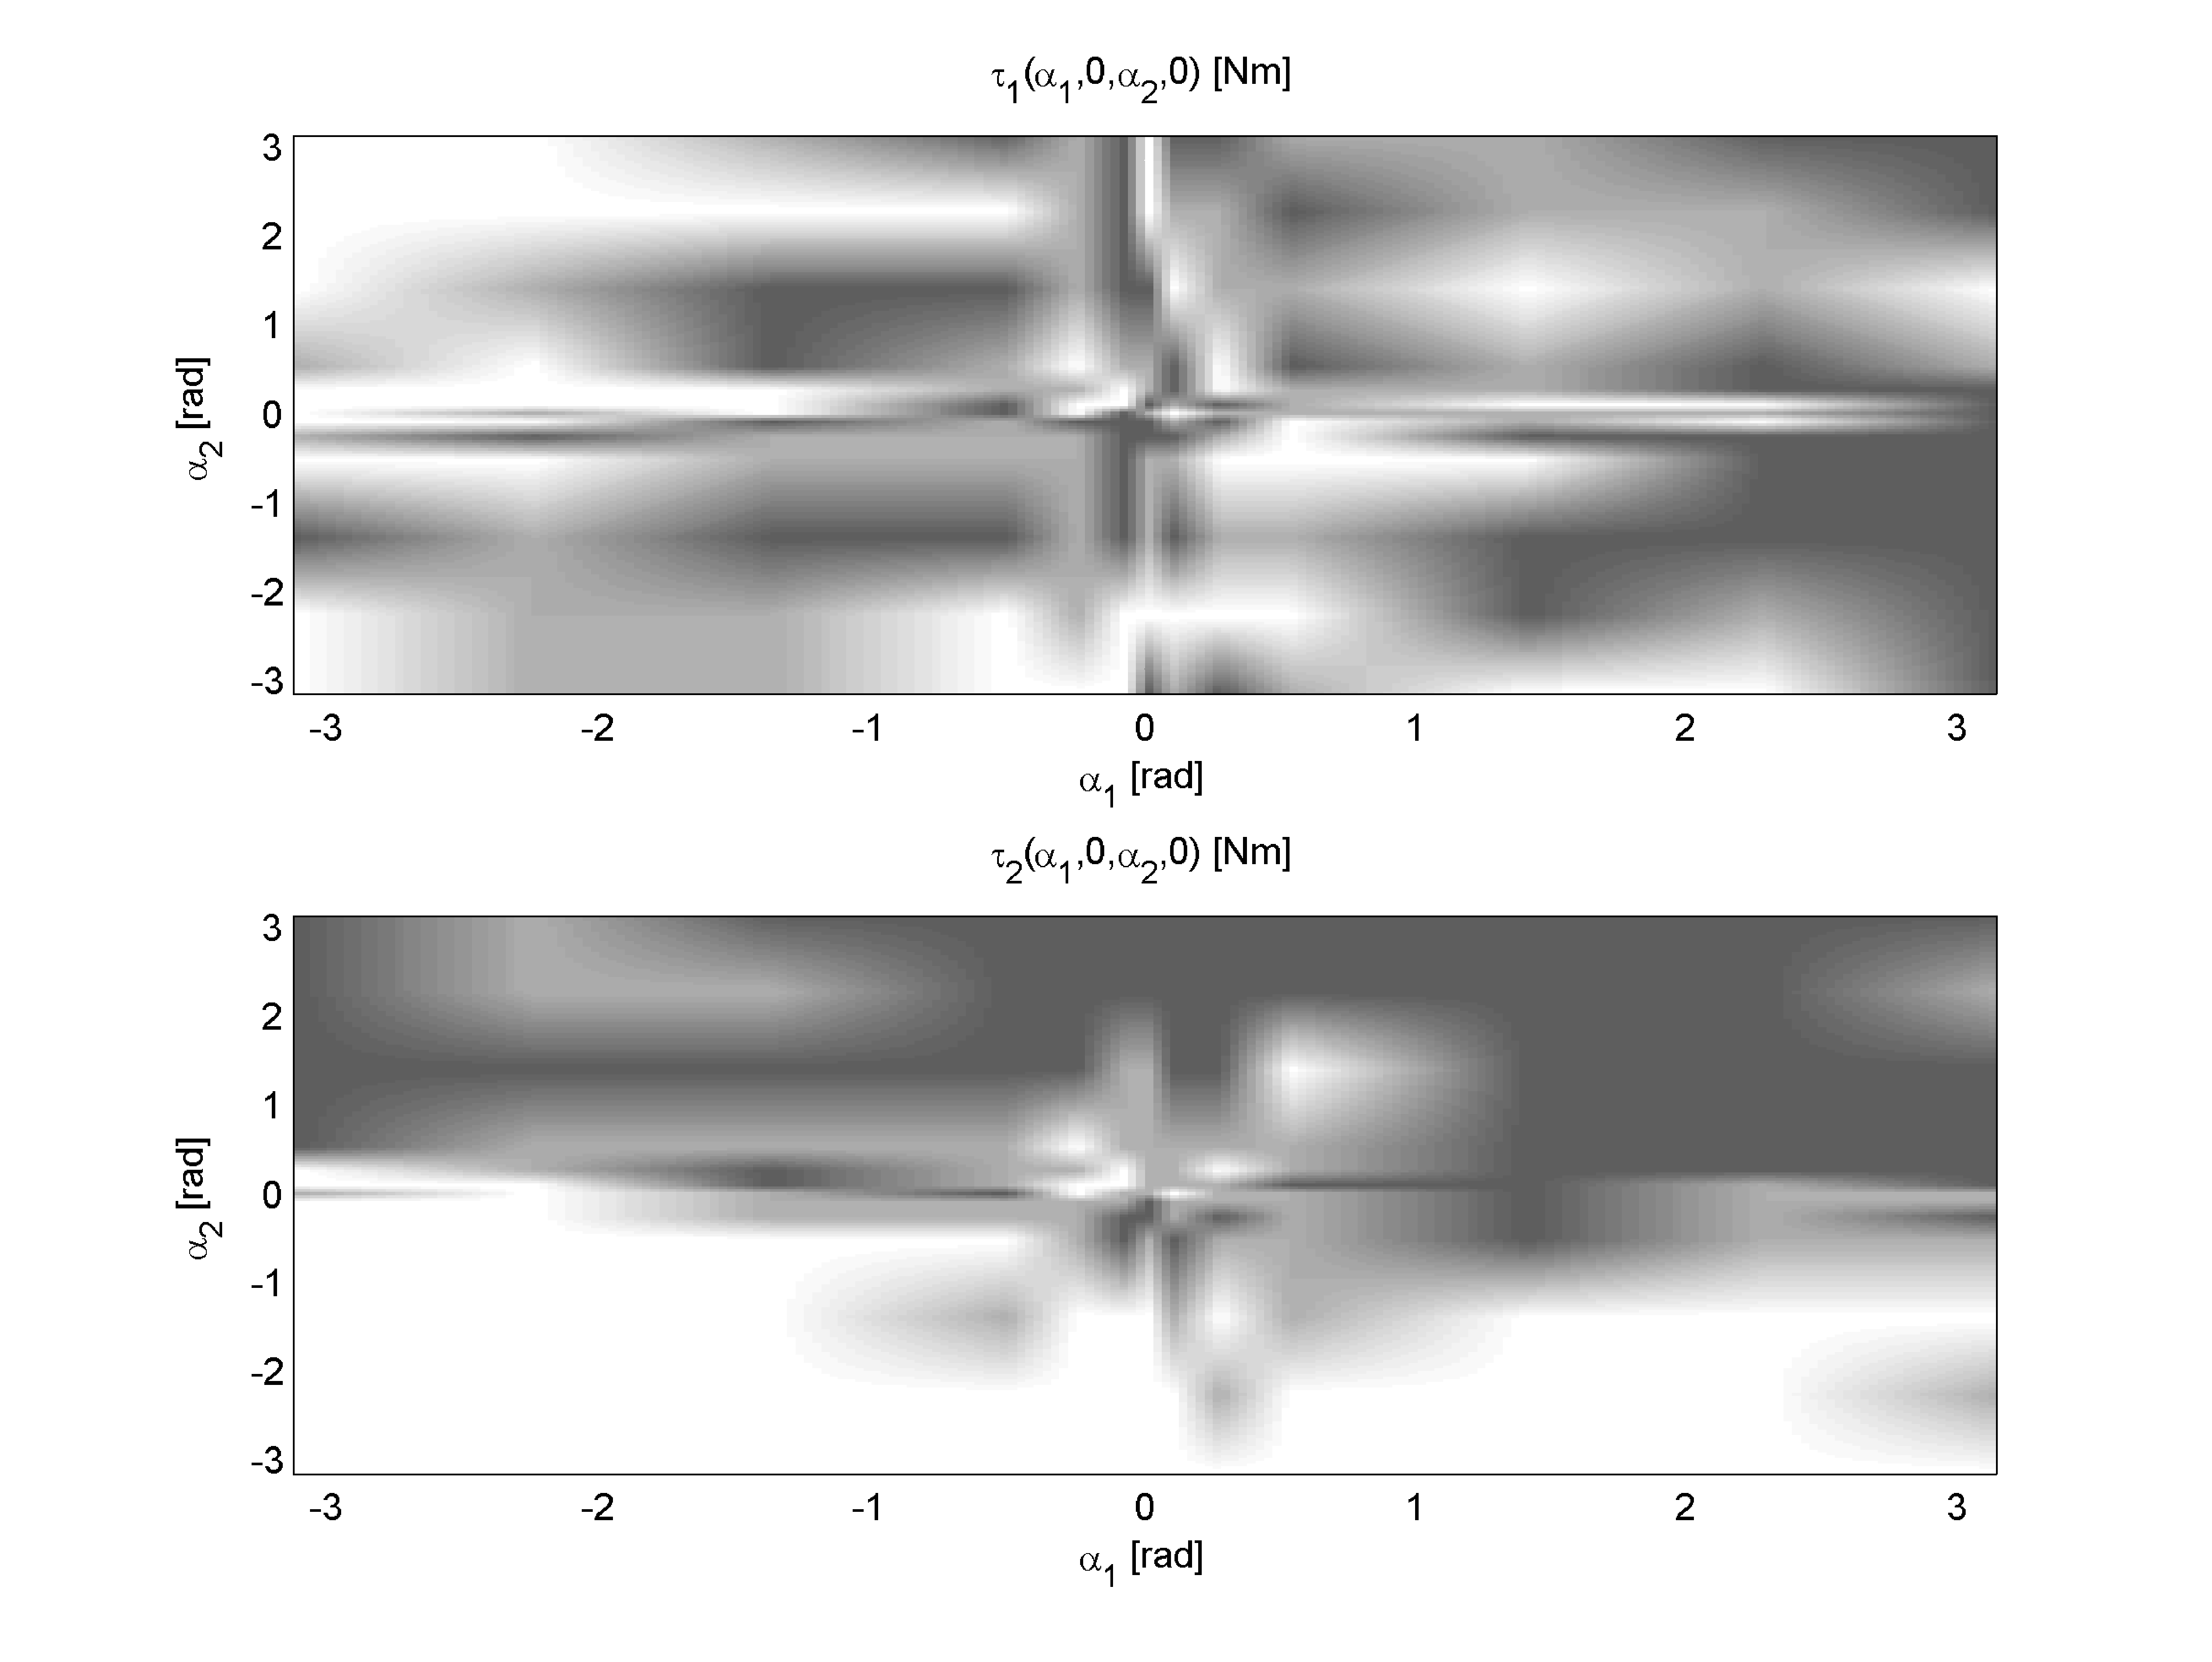
\includegraphics[width=.4\textwidth]{Figures/rarm_fzqi_LLR_test_1_noise_001_fuzzyh.eps}
	\label{fig:Q-iteration-subfig2b}
	}
	\\
	\subfigure[nonlinear model, noise ($\sigma^2=0.05$), $J=-149.6$]{
	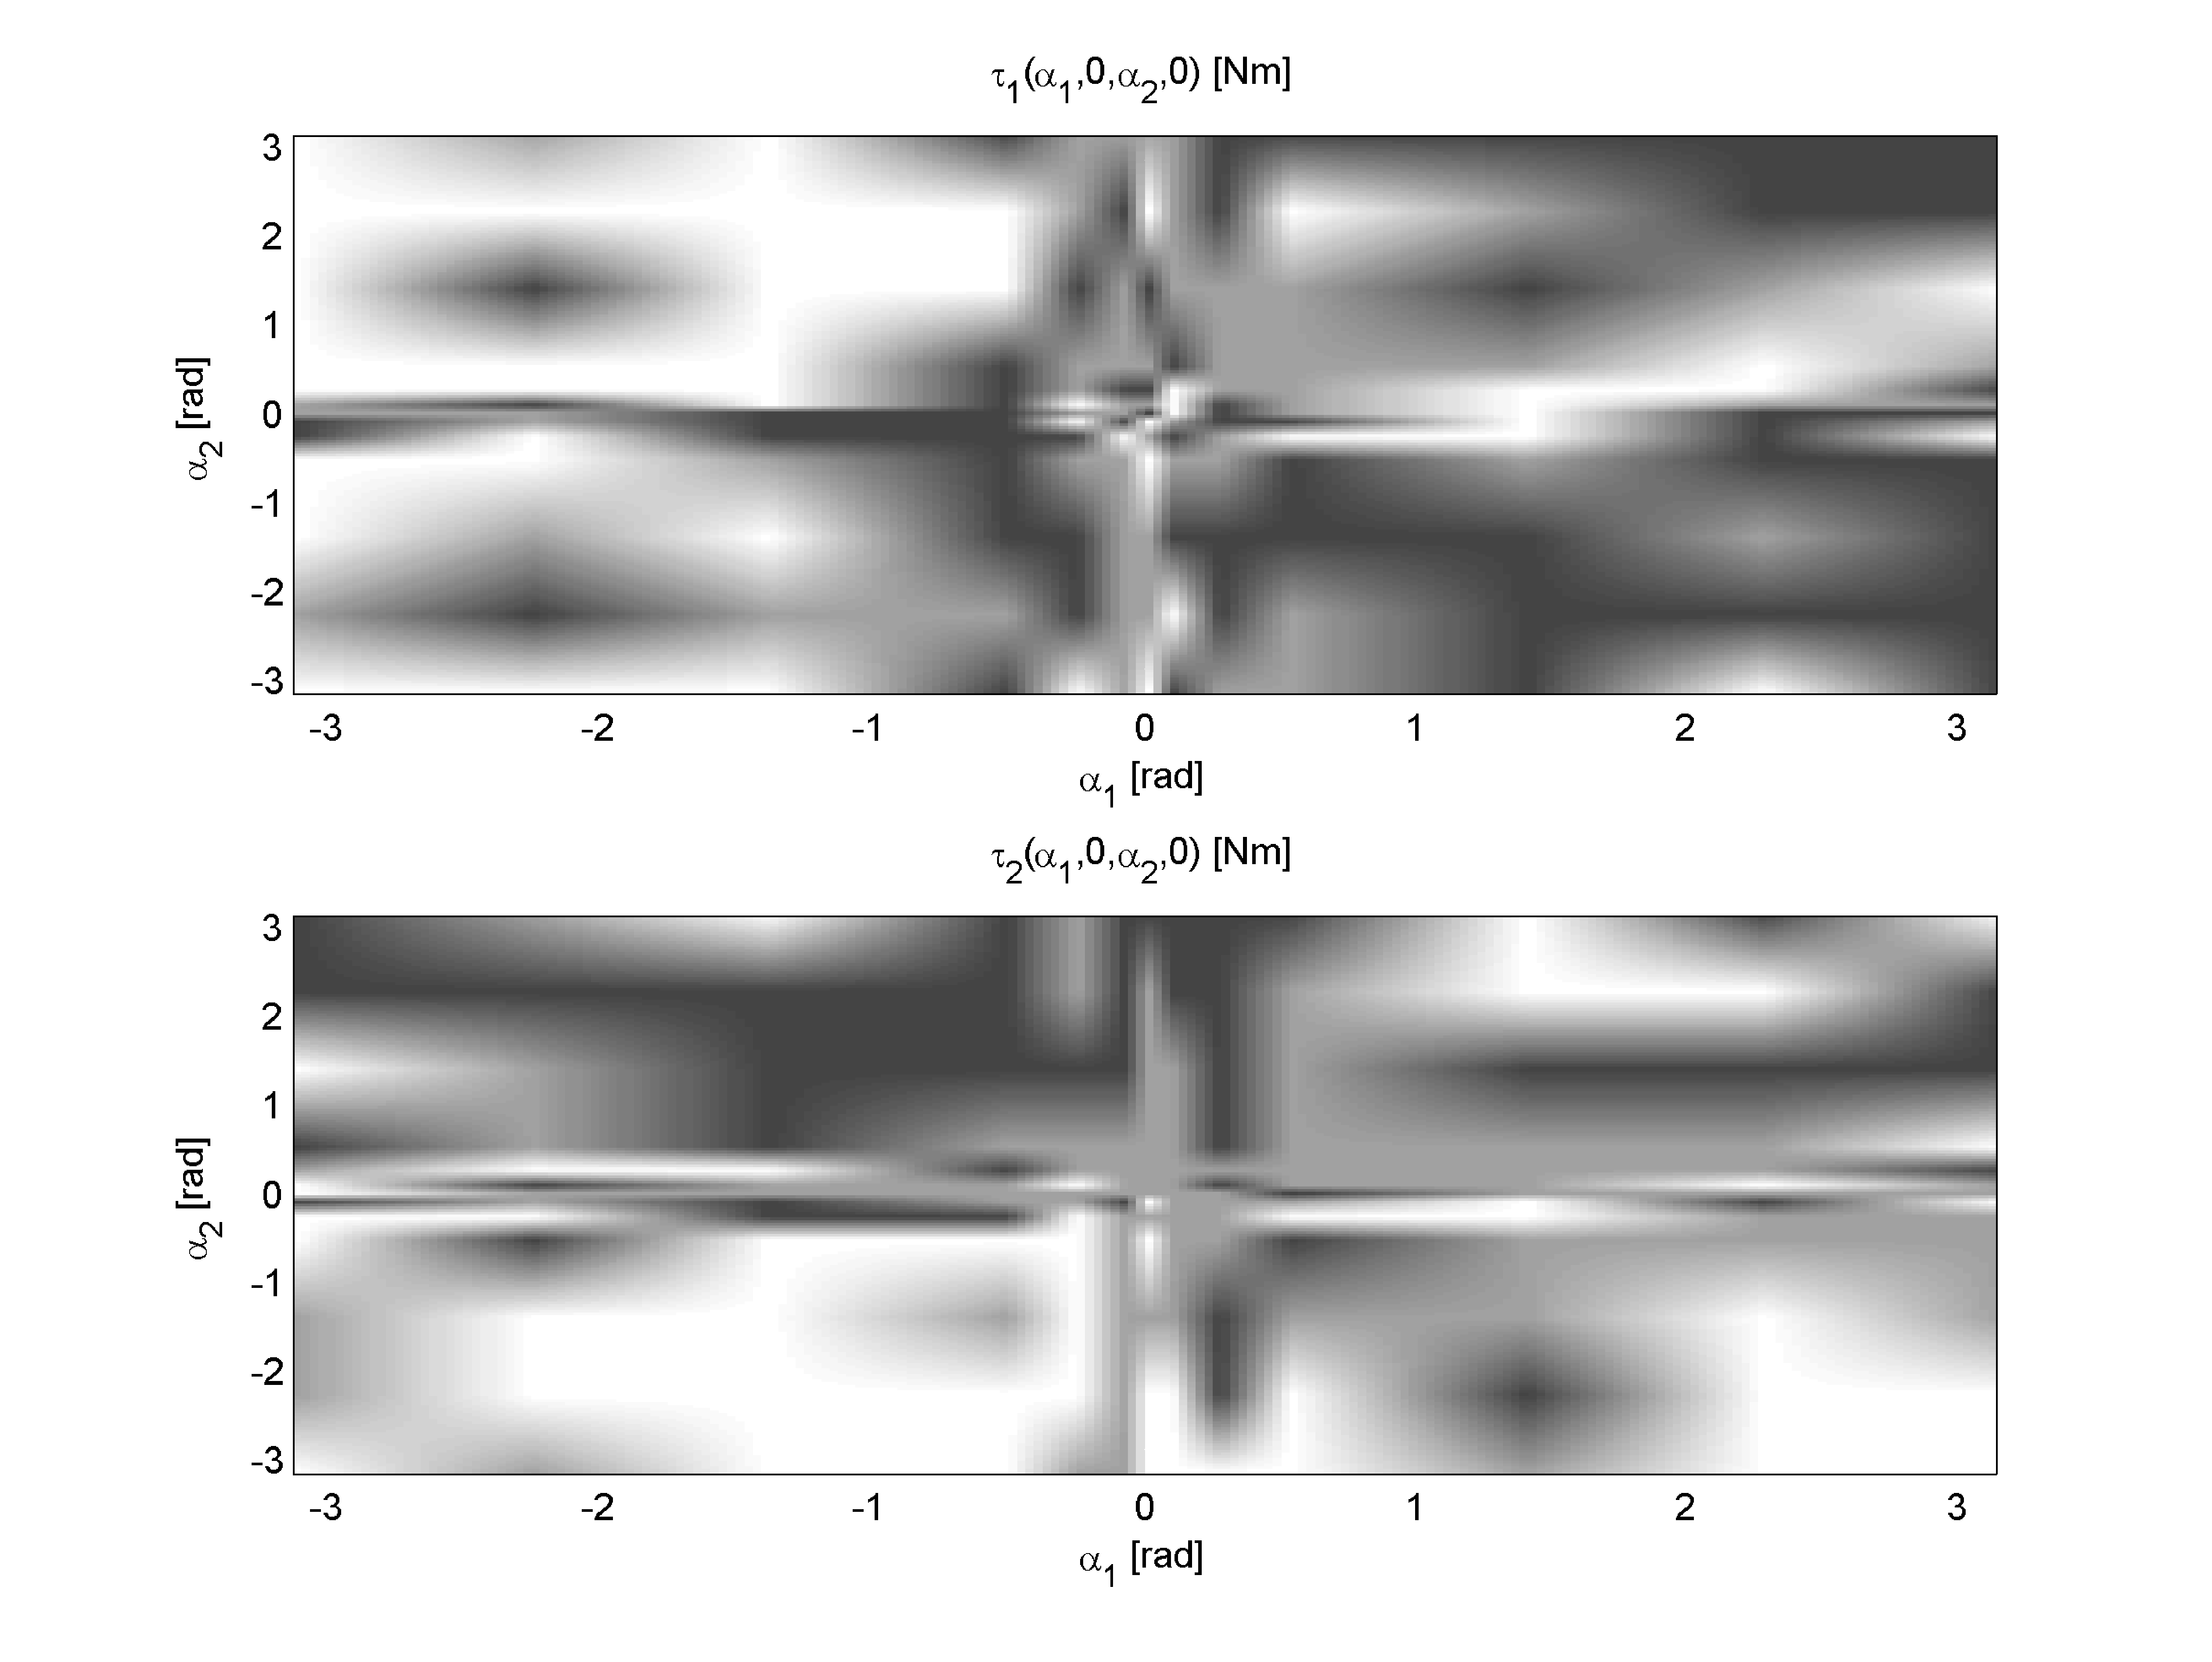
\includegraphics[width=.4\textwidth]{Figures/rarm_fzqi_test_1_noise_005_fuzzyh.eps}
	\label{fig:Q-iteration-subfig3a}
	}
	\subfigure[LLR model, noise ($\sigma^2=0.05$, $J=-202.6$]{
	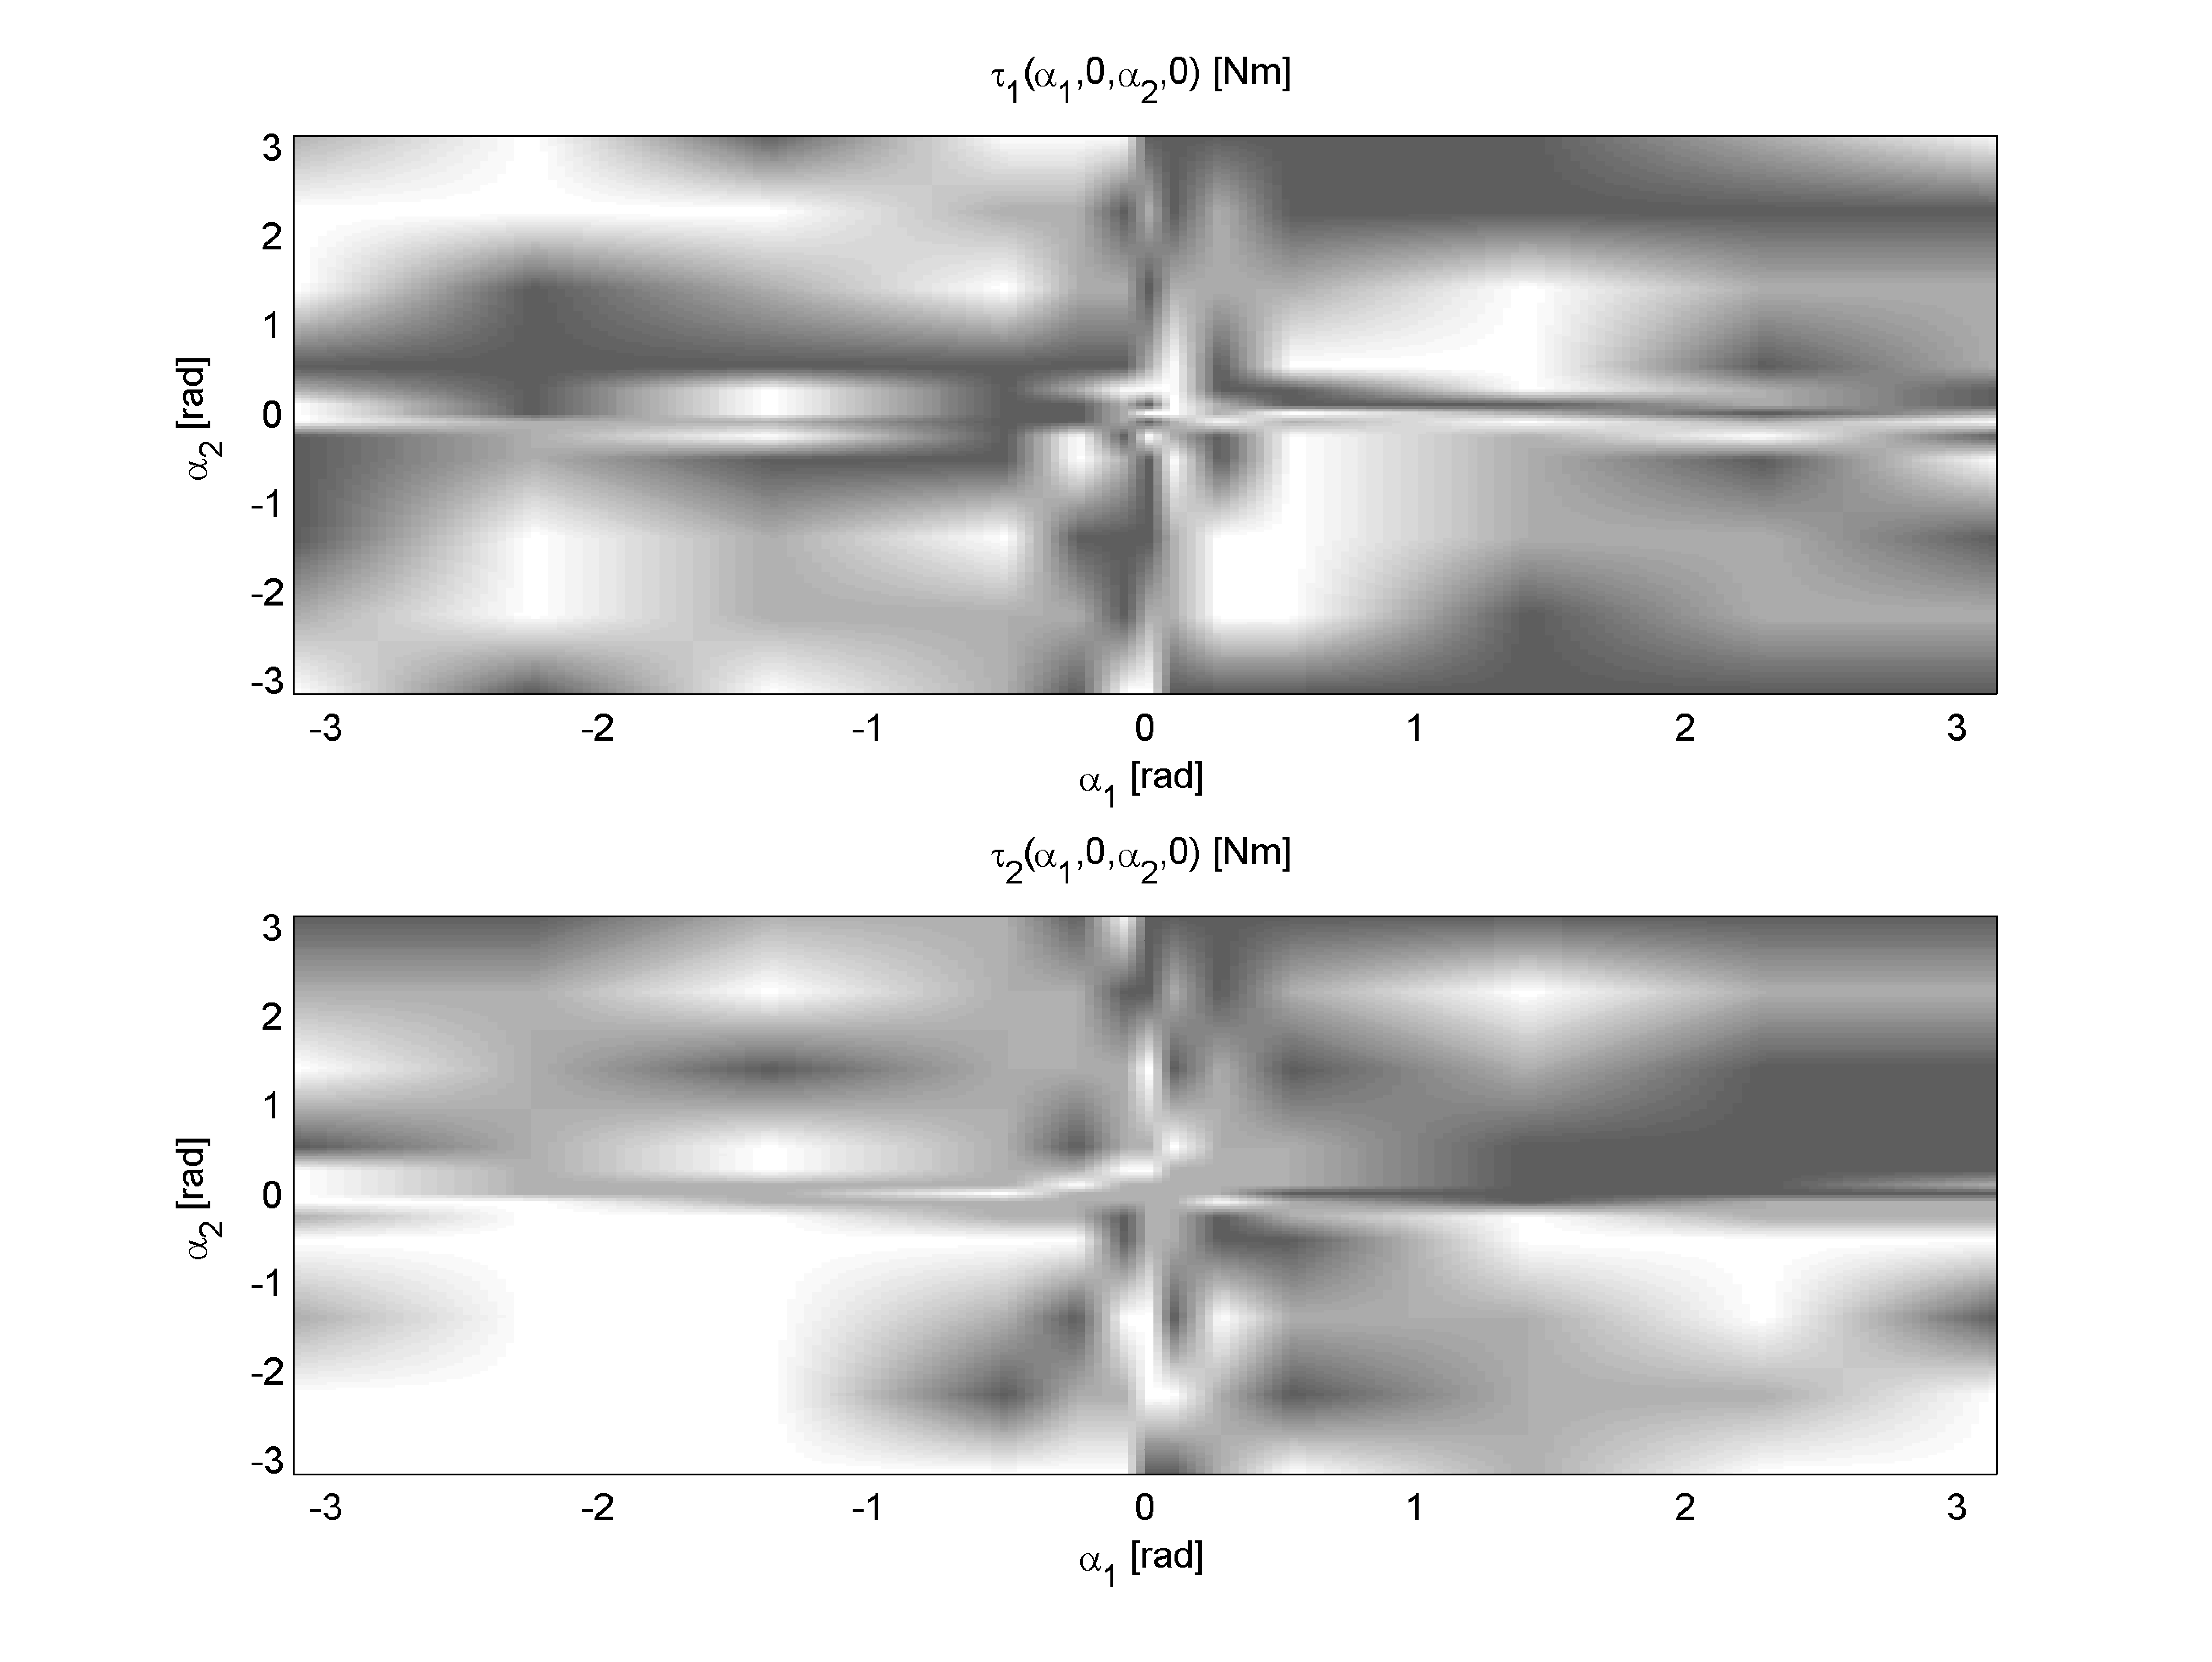
\includegraphics[width=.4\textwidth]{Figures/rarm_fzqi_LLR_test_1_noise_005_fuzzyh.eps}
	\label{fig:Q-iteration-subfig3b}
	}
	\caption[Q-iteration results]{Q-iteration policies for several settings with increasing noise. \ref{fig:Q-iteration-subfig1a}, \ref{fig:Q-iteration-subfig2a}, \ref{fig:Q-iteration-subfig3a} are the results for the nonlinear model; \ref{fig:Q-iteration-subfig1b}, \ref{fig:Q-iteration-subfig2b}, \ref{fig:Q-iteration-subfig3b} are for the \ac{LLR} estimate. The white, gray and black areas correspond to control voltages of +3V, 0 and -3V respectively.}
	\label{fig:Q-iteration-results}
\end{figure}

\section{Conclusion \& discussion}
We used Q-iteration to obtain results that could easily be compared for different parameters and could be used as benchmarks for the on-line learning learning methods. However, the results are not satisfactory. The results obtained with the \ac{LLR} model are far worse than those obtained with the nonlinear model. Also the number of memory samples needed was very high. Much higher than when \ac{LLR} was used to estimate trajectories.

Although Q-iteration has advantages over an on-line learning method because it limits the number of tuning/learning parameters, it might not be the best setting to test \ac{LLR}. Especially in view of the final application of the model: application of \ac{LLR} in a Dyna/\ac{PS} setting. The model will not be used to model the entire state-space, but only certain parts (the parts that have been visited by the agent and trajectories that lead to high rewards). In Q-iteration one assumes complete knowledge of the entire state-space.


